\documentclass[english, aspectratio=169]{beamer}
% english is for the language used in standard texts (figures, tables etc)
% aspectratio of 16:9 or set it for more old school to 4:3 (without the ':')

% ---------------------------------------------------------------------------- %
% Load base preamble
% ---------------------------------------------------------------------------- %
\usepackage{import}
\subimport{./preamble/}{beamer.tex}

\metroset{sectionpage=none}

% ---------------------------------------------------------------------------- %
% Local settings
% ---------------------------------------------------------------------------- %
% https://tex.stackexchange.com/a/20613
\newcommand\hcancel[2][black]{\setbox0=\hbox{$#2$}%
  \rlap{\raisebox{.35\ht0}{\textcolor{#1}{\rule{\wd0}{1pt}}}}#2}

\newcommand{\B}[0]{\ensuremath{\mathbb{B}}}

\newcommand{\sort}[0]{\text{sort}}

\newcommand{\triple}[3]{\ensuremath{(#1, #2, #3)}}
\renewcommand{\arc}[3]{\ensuremath{#1 \xrightarrow{_{#2}} #3}}

% ------------------------------------------------------------------------------
% TITLEPAGE
% ------------------------------------------------------------------------------
\title{Random Access on Narrow Decision Diagrams\\in External Memory}

\author{
  {\bf Steffan Christ S{\o}lvsten},
  Casper Moldrup Rysgaard,
  and Jaco van de Pol
}

\institute{\includegraphics[width=0.2\linewidth]{external/aulogo_uk_var2_black.eps}}

\date{SPIN 2024}

\begin{document}

\titleframe

\input{fram/adiar.tex}

\begin{frame}
  \only<1>{
    \setvalue{feature = black}
    \setvalue{optimisations = gray}
  }
  \only<2>{
    \setvalue{feature = gray}
    \setvalue{optimisations = black}
  }

  \begin{center}
    \fontsize{32}{60}\selectfont

    \begin{tabular}{cl}
      \color{\getvalue{feature}} \faIcon{tasks} & \color{\getvalue{feature}} \textbf{Features}
      \\
      \color{\getvalue{optimisations}} \faIcon{tools} & \color{\getvalue{optimisations}} \textbf{Optimisations}
    \end{tabular}
  \end{center}
\end{frame}

\blankframe

\begin{frame}
  \vspace{29pt}

  \begin{figure}
    \centering

    \begin{subfigure}{1.0\linewidth}
      \centering

      \begin{subfigure}[b]{0.46\linewidth}
        \centering

        \begin{tikzpicture}[scale=0.95, every node/.style={transform shape}]
          \input{tikz/bdd_example_a.tex}
        \end{tikzpicture}
      \end{subfigure}
      \begin{subfigure}[b]{0.53\linewidth}
        \centering
        { \footnotesize
          \begin{tabular}{r c l}
            [ & $\triple{(0,0)}{(2,0)}{(1,0)}$ & ,
            \\ \\
              & $\triple{(1,0)}{(2,0)}{(3,1)}$ & ,
            \\ \\
              & $\triple{(2,0)}{(3,0)}{(3,1)}$ & ,
            \\ \\
              & $\triple{(3,0)}{\top}{\bot}$   & ,
            \\ \\
              & $\triple{(3,1)}{\bot}{\top}$   & ]
          \end{tabular}
          \vspace{6pt}
        }
      \end{subfigure}

      \caption{$(x_0 \wedge x_1 \wedge x_3) \vee (x_2 \oplus x_3)$}
    \end{subfigure}
    \caption{Serialized Representation of a Binary Decision Diagram.}
  \end{figure}
\end{frame}

\begin{frame}
  \input{anim/count_paths_tfp.tex}
\end{frame}

\begin{frame}
  \begin{figure}
    \centering

    \begin{tikzpicture}[scale=0.8]
      \onslide<2-> {
        \node[shape = circle, draw = black] (s) {\small $(i,s)$};
      }

      % First node
      \onslide<3-> {
        \node[shape = circle, draw = black, below left=3 and 2 of s] (t) {\small $(j,t)$};

        \node[below left  = 0.5 and 0.2 of t] (alpha) {$\alpha$};
        \node[below right = 0.5 and 0.2 of t] (beta)  {$\beta$};

        \draw[->, dashed] (t) edge (alpha);
        \draw[->] (t) edge (beta);
      }

      \onslide<3->{
        \draw[->, densely dotted, thick](s) edge[bend right] node[above left] {$\texttt{PQ}_{1}$} (t);
      }

      % Second node
      \onslide<4-> {
        \node[below=3 of s] {\small $\cdots$};

        \node[shape = circle, draw = black, below right=3 and 2 of s] (u) {\small $(j,u)$};

        \node[below left  = 0.5 and 0.2 of u] (gamma) {$\gamma$};
        \node[below right = 0.5 and 0.2 of u] (delta) {$\delta$};

        \draw[->, dashed] (u) edge (gamma);
        \draw[->] (u) edge (delta);
      }

      \onslide<5> {
        \draw[->, densely dotted, thick] (t) edge[bend left] node[above] {$\texttt{PQ}_{2}$} (u);
      }
      \onslide<6-> {
        \draw[->, lightgray, densely dotted, thick] (t) edge[bend left] node[above] {$\texttt{PQ}_{2}$} (u);

        \node[red, opacity=0.8] at (-0.07,-3.3) {\fontsize{42}{0} \faIcon{times}};
        \node[red, opacity=0.8] at (-0.07,-4.5) {\Large\bf[SPIN 24]};
      }
    \end{tikzpicture}
  \end{figure}
\end{frame}

\begin{frame}
  \begin{figure}
    \centering

    \begin{tikzpicture}[baseline=-75pt]
      \onslide<2> {
        \draw[draw=red, thick, opacity=0.7] (-1.7,0.55) rectangle ++(3.4,-4.0);
      }

      \onslide<4> {
        \draw[draw=red, thick, opacity=0.7] (-1.7, 0.51) rectangle ++(3.4,-0.99);
      }
      \onslide<5> {
        \draw[draw=red, thick, opacity=0.7] (-1.7,-0.47) rectangle ++(3.4,-0.99);
      }
      \onslide<6> {
        \draw[draw=red, thick, opacity=0.7] (-1.7,-1.44) rectangle ++(3.4,-0.98);
      }
      \onslide<7> {
        \draw[draw=red, thick, opacity=0.7] (-1.7,-2.40) rectangle ++(3.4,-0.99);
      }

      \onslide<8> {
        % dummy
      }
      \onslide<9> {
        \draw[draw=red, dashed, thick, opacity=0.7] (-1.7,-2.40) rectangle ++(3.4,-0.99);
      }

      \input{tikz/bdd_example_a.uid.tex}
    \end{tikzpicture}
    \qquad\qquad
    \onslide<9> {
      { \LARGE\color{red}
        \begin{tabular}{c}
          \faIcon{ruler}
          \\
          \normalsize Width
          \\ \hline
          2
        \end{tabular}
      }
    }
  \end{figure}
\end{frame}

\blankframe

\begin{frame}
  \begin{figure}
    \centering

    \begin{subfigure}[b]{0.5\linewidth}
      \begin{tikzpicture}
        \begin{axis}[%
          width=0.96\linewidth, height=0.75\linewidth,
          every tick label/.append style={font=\scriptsize},
          % x-axis
          xlabel={Problem Complexity (N)},
          xtick={14,15,16,17},
          xmajorgrids=true,
          xmin=13.5,
          xmax=16.5,
          % y-axis
          ymin=100,
          ymax=100000,
          ymode=log,
          ytick={10,100,1000,10000,100000,1000000},
          ylabel={Time (s)},
          yminorgrids=false,
          ymajorgrids=true,
          grid style={dashed,black!20},
          ]

          \colorlet{adiar}{red}
          \colorlet{cudd}{orange}

          \tikzstyle{plot_adiar}=[color=adiar, mark=diamond*, mark size=2pt, line width=1pt,
                                  mark options={color=adiar, fill=adiar, opacity=0.6}]
          \tikzstyle{plot_cudd}=[color=cudd, mark=triangle*, mark size=2pt, line width=1pt,
                                 mark options={color=cudd, fill=cudd, opacity=0.6}]


          \addplot [style=plot_cudd] coordinates {
            (13, 52.881)
            (14, 316.093)
            (15, 2687.585)
          };

          \only<2> {
            \addplot [style=plot_adiar] coordinates {
              (13, 118.887)
              (14, 660.127)
              (15, 3943.981)
              (16, 31017.033)
              (17, 265758.859)
            };
          }

          \only<3> {
            \addplot [style=plot_adiar] coordinates {
              (13, 82.715)
              (14, 502.855)
              (15, 3336.591)
              (16, 23127.559)
              (17, 196813.872)
            };
          }

          \only<4> {
            \addplot [style=plot_adiar] coordinates {
              (13, 71.277)
              (14, 434.766)
              (15, 2855.766)
              (16, 19400.135)
              (17, 202684.356)
            };
          }
        \end{axis}
      \end{tikzpicture}
    \end{subfigure}
    \begin{subfigure}[b]{0.49\linewidth}
      \centering

      \large
      \begin{tabular}[b]{cll c c}
                                  &       &                             &   & \faIcon{stopwatch}
        \\
                                  &       &                             &   & \normalsize $N = 15$
        \\ \hline
        {\color{orange} $\triangle$} & CUDD  & v3.0                        & : & 44.8 min%
        \onslide<2-> {
        \\ \hline
        {\color{red} $\diamond$}  & Adiar & v1.0                        & : & 66.7 min}%
        \onslide<3-> {
        \\
                                  & \multicolumn{2}{l}{+ cuts}          & : & 56.8 min}%
        \onslide<4-> {
        \\
                                  & \multicolumn{2}{l}{+ random access} & : & 47.2 min}%
      \end{tabular}

      \vspace{27pt}
    \end{subfigure}

    \caption{\Large Queens | 300 GiB of RAM}
  \end{figure}
\end{frame}

\begin{frame}
  \begin{figure}
    \centering

    \begin{subfigure}[b]{0.7\linewidth}
      \centering

      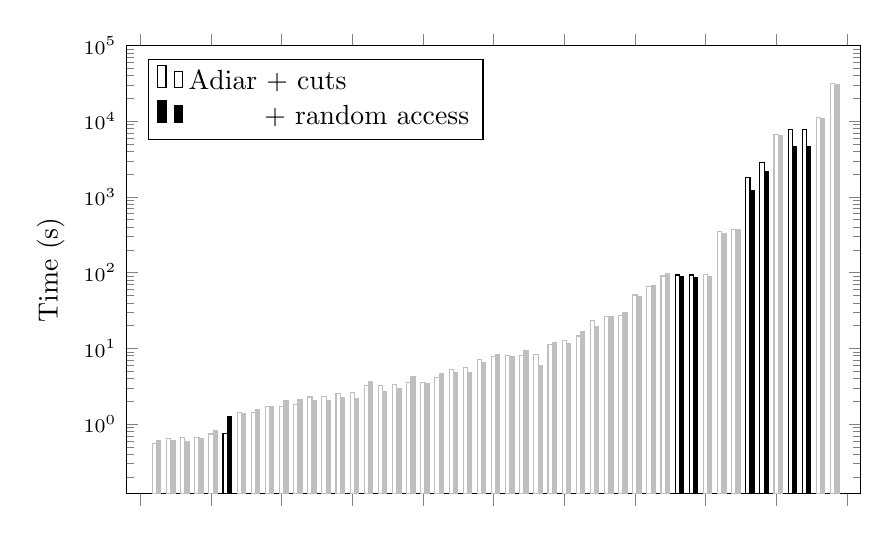
\begin{tikzpicture}
        \begin{axis}[
          ybar,
          bar width = 0.3,
          % x axis
          xmin=-1,
          xmax=51,
          xticklabel=\empty,
          % y axis
          every tick label/.append style={font=\scriptsize},
          ymin=0.12,
          ymax=100000,
          ymode=log,
          ylabel={Time (s)},
          log origin=infty,
          % dimensions
          width=0.9\linewidth,
          height=0.6\linewidth,
          % legend
          legend cell align=left,
          legend pos=north west,
          legend style={draw=black,fill=white}
          ]

          % --------------------------------------------------
          % Insignificant

          % Before
          \addplot[draw=lightgray, bar shift=0.0, forget plot] coordinates {
            (1, 0.553)
            (2, 0.648)
            (3, 0.669)
            (4, 0.672)
            (5, 0.741)
            (7, 1.428)
            (8, 1.430)
            (9, 1.688)
            (10, 1.692)
            (11, 1.813)
            (12, 2.284)
            (13, 2.326)
            (14, 2.533)
            (15, 2.586)
            (16, 3.212)
            (17, 3.213)
            (18, 3.335)
            (19, 3.510)
            (20, 3.531)
            (21, 4.136)
            (22, 5.329)
            (23, 5.570)
            (24, 7.146)
            (25, 7.896)
            (26, 8.031)
            (27, 8.073)
            (28, 8.331)
            (29, 11.112)
            (30, 12.552)
            (31, 14.580)
            (32, 23.515)
            (33, 26.727)
            (34, 27.478)
            (35, 50.700)
            (36, 65.379)
            (37, 90.475)
            (40, 94.926)
            (41, 353.040)
            (42, 374.774)
            (45, 6763.235)
            (48, 11110.969)
            (49, 31356.054)
          };
          % After
          \addplot[draw=lightgray, fill=lightgray, bar shift=0.3, forget plot] coordinates {
            (1, 0.604)
            (2, 0.608)
            (3, 0.595)
            (4, 0.648)
            (5, 0.835)
            (7, 1.373)
            (8, 1.576)
            (9, 1.712)
            (10, 2.071)
            (11, 2.117)
            (12, 2.025)
            (13, 2.055)
            (14, 2.271)
            (15, 2.158)
            (16, 3.625)
            (17, 2.654)
            (18, 2.965)
            (19, 4.215)
            (20, 3.468)
            (21, 4.713)
            (22, 4.761)
            (23, 4.754)
            (24, 6.517)
            (25, 8.355)
            (26, 7.832)
            (27, 9.491)
            (28, 5.927)
            (29, 11.970)
            (30, 11.535)
            (31, 16.853)
            (32, 19.186)
            (33, 26.271)
            (34, 29.663)
            (35, 48.747)
            (36, 66.961)
            (37, 98.239)
            (40, 90.200)
            (41, 327.385)
            (42, 375.640)
            (45, 6559.876)
            (48, 10918.547)
            (49, 30889.871)
          };

          % --------------------------------------------------
          % Significant

          % Before
          \addplot[draw=black, bar shift=0.0] coordinates {
            (6, 0.744)
            (38, 93.063)
            (39, 93.212)
            (43, 1832.058)
            (44, 2885.936)
            (46, 7780.512)
            (47, 7832.249)
          };
          % After
          \addplot[color=black, fill=black, bar shift=0.3] coordinates {
            (6, 1.241)
            (38, 87.987)
            (39, 86.588)
            (43, 1201.214)
            (44, 2152.830)
            (46, 4660.012)
            (47, 4644.692)
          };

          % --------------------------------------------------
          \legend{Adiar + cuts, \hspace{24pt} + random access}
        \end{axis}
      \end{tikzpicture}
    \end{subfigure}
    \begin{subfigure}[b]{0.29\linewidth}
      \begin{tabular}[b]{c}
        \faIcon{chevron-up}
        \\
        Speed Ups
        \\ \hline
        6 (+26.9\%)
        \\
        \\
        \faIcon{chevron-down}
        \\
        Slowdowns
        \\ \hline
        1 (-66.8\%)
      \end{tabular}

      \vspace{20pt}
    \end{subfigure}

    \caption{\Large EPFL Circuit Verification | 300 GiB of RAM}
  \end{figure}
\end{frame}

\blankframe

\input{fram/endslate.tex}

% ------------------------------------------------------------------------------ %
% APPENDIX
% ------------------------------------------------------------------------------ %
\begin{frame}
  \begin{figure}
    \centering

    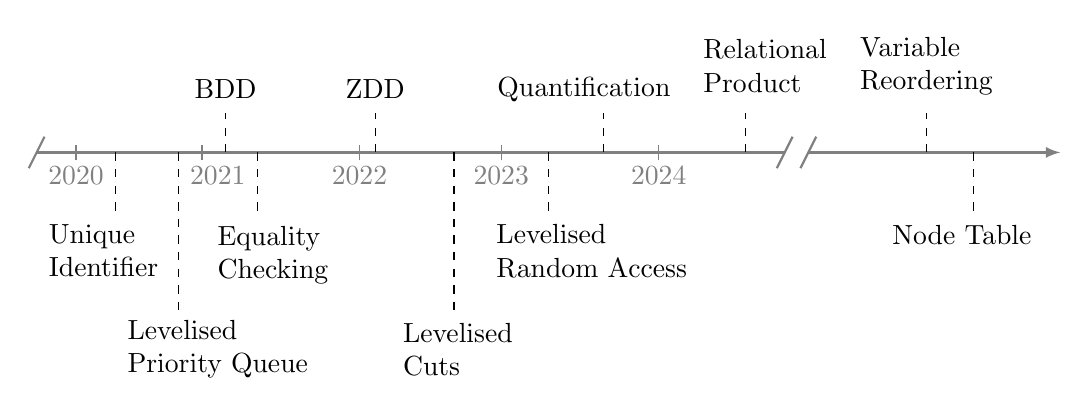
\begin{tikzpicture}
      % PhD line
\draw[gray][thick] (0.6,0.2) -- (0.4,-0.2);
\draw[gray][-, thick] (0.5,0) -- (10,0);
\draw[gray][thick] (10.1,0.2) -- (9.9,-0.2);

% 2021
\draw[gray] (1,-0.1) -- ++(0,0.2);
\node[gray] at (1,-0.3) {$2020$};

\draw[dashed, color=black] (1.5,0) -- ++(0,-0.8);
\node[color=black, align=left] at (1.35,-1.25)
{Unique\\Identifier};

\draw[dashed, color=black] (2.3,0) -- ++(0,-2.0);
\node[color=black, align=left] at (2.8,-2.5)
{Levelised\\Priority Queue};

% 2021
\draw[gray] (2.6,-0.1) -- ++(0,0.2);
\node[gray] at (2.8,-0.3) {$2021$};

\draw[dashed, color=black] (2.9,0) -- ++(0,0.5);
\node[color=black, align=left] at (2.9,0.8)
{BDD};

\draw[dashed, color=black] (3.3,0) -- ++(0,-0.8);
\node[color=black, align=left] at (3.5,-1.3)
{Equality\\Checking};

% 2022
\draw[gray] (4.6,-0.1) -- ++(0,0.2);
\node[gray] at (4.6,-0.3) {$2022$};

\draw[dashed, color=black] (4.8,0) -- ++(0,0.5);
\node[color=black, align=left] at (4.8,0.8)
{ZDD};

\draw[dashed, color=black] (5.8,0) -- ++(0,-2.0);
\node[color=black, align=left] at (5.85,-2.5)
{Levelised\\Cuts};

% 2023
\draw[gray] (6.4,-0.1) -- ++(0,0.2);
\node[gray] at (6.4,-0.3) {$2023$};

\draw[dashed, color=black] (7.0,0) -- ++(0,-0.8);
\node[color=black, align=left] at (7.55,-1.25)
{Levelised\\Random Access};

\draw[dashed, color=black] (7.7,0) -- ++(0,0.5);
\node[color=black, align=left] at (7.45,0.8)
{Quantification};

% 2024
\draw[gray] (8.4,-0.1) -- ++(0,0.2);
\node[gray] at (8.4,-0.3) (y2024) {$2024$};

\draw[dashed, color=black] (9.5,0) -- ++(0,0.5);
\node[color=black, align=left] at (9.75,1.1)
{Relational\\Product};

% Post PhD line
\draw[gray][thick] (10.4,0.2) -- (10.2,-0.2);
\draw[gray][-latex, thick] (10.3,0) -- (13.5,0);

\draw[dashed, color=black] (11.8,0) -- ++(0,0.5);
\node[color=black, align=left] at (11.8,1.1)
{Variable\\Reordering};

\draw[dashed, color=black] (12.4,0) -- ++(0,-0.8);
\node[color=black, align=left] at (12.25,-1.05)
{Node Table};

    \end{tikzpicture}
  \end{figure}
\end{frame}

\end{document}
